\documentclass[a4paper]{article}

\usepackage[margin=1in]{geometry}
\setlength\parindent{0pt}

\usepackage{mathtools}
\usepackage{enumitem} % enumeration label options
\usepackage{amsfonts} % \mathbb, ...
\usepackage{amsthm}
\usepackage{tikz}
\usepackage{caption}
\usepackage{subcaption}

\theoremstyle{plain}
\newtheorem{theorem}{Theorem}
\newtheorem{proposition}[theorem]{Proposition}
\newtheorem{lemma}[theorem]{Lemma}
\newtheorem{corollary}[theorem]{Corollary}

\theoremstyle{remark}
\newtheorem*{remark}{Remark}
\newtheorem*{example}{Example}
\newtheorem*{exercise}{Exercise}

\theoremstyle{definition}
\newtheorem*{definition}{Definition}
\newtheorem*{notation}{Notation}

\DeclareMathOperator{\ord}{ord}
\DeclareMathOperator{\res}{res}
\DeclareMathOperator{\ch}{char}

\newcommand{\divides}{\bigm|}

\renewcommand{\P}{\mathbb{P}}
\renewcommand{\O}{\mathcal{O}}
\newcommand{\E}{\mathcal{E}}
\newcommand{\F}{\mathbb{F}}
\newcommand{\N}{\mathbb{N}}
\newcommand{\Z}{\mathbb{Z}}
\newcommand{\Q}{\mathbb{Q}}
\newcommand{\R}{\mathbb{R}}
\newcommand{\C}{\mathbb{C}}

\title{Notes for ``Elliptic Curves'' by Vladimir Dokchitser}
\author{Calum Crossley}
\date{2023-2024}

\begin{document}

\maketitle

Preparatory information:
\begin{itemize}
    \item Books: Silverman's ``The Arithmetic of Elliptic Curves''
    \item Prerequisites: basics of Galois theory, basics of number fields,
        basics of algebraic curves, complex analysis, $p$-adic numbers
    \item Exercise sheets: 1 per lecture, 2 out of 5 exercises for assessment
        (marked with a ``+'')
    \item Lectures: 10 of them
\end{itemize}

Tentative lecture topics:
\begin{enumerate}[label=\arabic*)]
    \item The group law
    \item Elliptic curves over $\C$
    \item Heights
    \item The Mordell-Weil theorem
    \item Elliptic curves over $\Q_p$
    \item Formal groups
    \item Explicit 2-descent
    \item Tate modules
    \item $L$-functions and BSD
    \item Selmer groups
\end{enumerate}

\paragraph{Pre-waffle.}
This is a number theory course, so we care about solving Diophantine equations.
For example, what are the rational solutions of $x^2+y^2=1$?
\begin{equation*}
    x = \frac{2t}{t^2+1}, \quad y = \frac{t^2-1}{t^2+1}, \quad t\in\Q.
\end{equation*}
The general case is impossibly hard; it is formally undecidable. We will focus
on curves, such as one equation with two variables. Life is strongly affected by
the geometry over $\C$, where the curve is a closed orientable surface in
projective space.
\begin{itemize}
    \item Genus 0: The Riemann sphere; $\P^1$. The number theory is easy; either
        there are no $\Q$-solutions or infinitely many nicely parametrized, and
        we can decide which (Hasse principle).

    \item Genus 1 (this course): The torus. There can be no $\Q$-solutions, or
        finitely many, or infinitely many. No proven algorithm exists for the
        general case, although there are algorithms conditional on the
        Tate--Shafarevich conjecture or the BSD conjecture.

    \item Genus $\ge2$: There are finitely many $\Q$-solutions by a theorem of
        Faltings.
\end{itemize}

\begin{remark}
    By Siegel's theorem there are only finitely many $\Z$-solutions for $g\ge1$.
\end{remark}

\section{Group Law}

\begin{definition}
    An \emph{elliptic curve} over a field $K$ is a projective non-singular curve
    $E$ of genus 1 over $K$, together with a given $K$-rational point $\O$.
\end{definition}

\begin{example}
    Take $E:y^2=x^3-x$, that is $Y^2Z=X^3-XZ^2$, with $\O=[0:1:0]$ the
    point at infinity.
\end{example}

\begin{definition}
    A \emph{(generalized) Weierstrass equation} over $K$ is an equation of the
    form
    \begin{equation*}
        Y^2Z + a_1XYZ + a_3YZ^2 = X^3 + a_2X^2Z + a_4XZ^2 + a_6Z^3
    \end{equation*}
    with $a_i\in K$. For ease of notation we identify this with the affine
    equation
    \begin{equation*}
        y^2 + a_1xy + a_3y = x^3 + a_2x^2 + a_4x + a_6.
    \end{equation*}
\end{definition}

\begin{remark}
    At infinity we have the point $[0:1:0]$ and no others. This is the standard
    choice for $\O$. If $E$ is non-singular, the genus is 1.
\end{remark}

\begin{notation}
    We write
    \begin{align*}
        E(K)
            &= \{\text{solutions $[X:Y:Z]$ to the equation over $K$}\} \\
            &= \{\O\}\cup\{\text{solutions $(x,y)$ to the equation over $K$}\}.
    \end{align*}
\end{notation}

\begin{example}
    If $E:y^2=f(x)$ with $f(x)$ a monic cubic, then $E(\R)$ looks as follows:
    \begin{figure}[htb]
        \centering
        \begin{subfigure}{0.25\textwidth}
            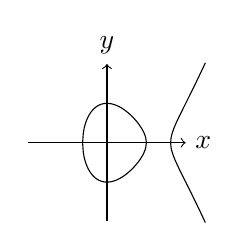
\begin{tikzpicture}
                \draw[->]
                    (-1,0) -- (1,0) node[right] {$x$};
                \draw[->]
                    (0,-1) -- (0,1) node[above] {$y$};
                \draw[scale=0.5,samples=100,domain=-0.618:1,variable=\x]
                    plot ({\x},{sqrt(abs(\x*\x*\x-2*\x*\x+1))});
                \draw[scale=0.5,samples=100,domain=1.618:2.5,variable=\x]
                    plot ({\x},{sqrt(abs(\x*\x*\x-2*\x*\x+1))});
                \draw[scale=0.5,samples=100,domain=-0.618:1,variable=\x]
                    plot ({\x},{-sqrt(abs(\x*\x*\x-2*\x*\x+1))});
                \draw[scale=0.5,samples=100,domain=1.618:2.5,variable=\x]
                    plot ({\x},{-sqrt(abs(\x*\x*\x-2*\x*\x+1))});
            \end{tikzpicture}
        \end{subfigure}
        \begin{subfigure}{0.25\textwidth}
            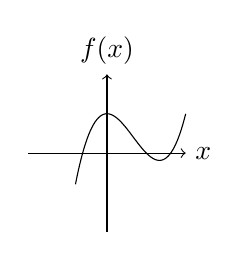
\begin{tikzpicture}
                \draw[->]
                    (-1,0) -- (1,0) node[right] {$x$};
                \draw[->]
                    (0,-1) -- (0,1) node[above] {$f(x)$};
                \draw[scale=0.5,domain=-0.8:2,samples=100,variable=\x]
                    plot ({\x},{\x*\x*\x-2*\x*\x+1});
            \end{tikzpicture}
        \end{subfigure}

        \medskip
        \begin{subfigure}{0.25\textwidth}
            \begin{tikzpicture}
                \draw[->]
                    (-1,0) -- (1,0) node[right] {$x$};
                \draw[->]
                    (0,-1) -- (0,1) node[above] {$y$};
                \draw[scale=0.5,samples=100,domain=1.678:2.5,variable=\x]
                    plot ({\x},{sqrt(abs(\x*\x*\x-1.5*\x*\x-0.5))});
                \draw[scale=0.5,samples=100,domain=1.678:2.5,variable=\x]
                    plot ({\x},{-sqrt(abs(\x*\x*\x-1.5*\x*\x-0.5))});
            \end{tikzpicture}
        \end{subfigure}
        \begin{subfigure}{0.25\textwidth}
            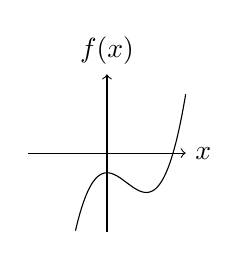
\begin{tikzpicture}
                \draw[->]
                    (-1,0) -- (1,0) node[right] {$x$};
                \draw[->]
                    (0,-1) -- (0,1) node[above] {$f(x)$};
                \draw[scale=0.5,domain=-0.8:2,samples=100,variable=\x]
                    plot ({\x},{\x*\x*\x-1.5*\x*\x-0.5});
            \end{tikzpicture}
        \end{subfigure}

        \medskip
        \begin{subfigure}{0.25\textwidth}
            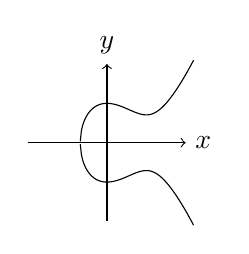
\begin{tikzpicture}
                \draw[->]
                    (-1,0) -- (1,0) node[right] {$x$};
                \draw[->]
                    (0,-1) -- (0,1) node[above] {$y$};
                \draw[scale=0.5,samples=100,domain=-0.678:2.2,variable=\x]
                    plot ({\x},{sqrt(abs(\x*\x*\x-1.5*\x*\x+1))});
                \draw[scale=0.5,samples=100,domain=-0.678:2.2,variable=\x]
                    plot ({\x},{-sqrt(abs(\x*\x*\x-1.5*\x*\x+1))});
            \end{tikzpicture}
        \end{subfigure}
        \begin{subfigure}{0.25\textwidth}
            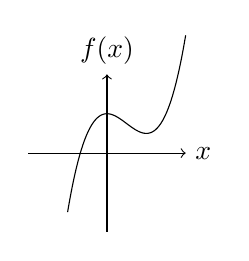
\begin{tikzpicture}
                \draw[->]
                    (-1,0) -- (1,0) node[right] {$x$};
                \draw[->]
                    (0,-1) -- (0,1) node[above] {$f(x)$};
                \draw[scale=0.5,samples=100,domain=-1:2,variable=\x]
                    plot ({\x},{\x*\x*\x-1.5*\x*\x+1});
            \end{tikzpicture}
        \end{subfigure}
    \end{figure}
\end{example}

\begin{theorem}[see Silverman, Chapter III]
    Let $\E$ be an elliptic curve over $K$. Then there exists an isomorphism (of
    projective varieties) from $\E$ to the projective curve defined by
    \begin{equation*}
        E : y^2 + a_1xy + a_3y = x^3 + a_2x^2 + a_4x + a_6
    \end{equation*}
    for some $a_i\in K$, mapping the given $K$-rational point to the point at
    infinity.
\end{theorem}

\begin{remark}
    To keep track of the indices for the Weierstrass equation, give $x$ weight
    2, $y$ weight 3, and $a_i$ weight $i$. The terms all have weight 6.
\end{remark}

\begin{example}
    Take $\E:y^2=x^4-1$ with point $P=(1,0)$.
    \begin{itemize}
        \item Let $x_2=x-1$, giving $y^2=x_2(x_2+2)(x_2^2+2x_2+2)$. (Move $P$ to
            the origin.)
        \item Let $x_3=1/x_2$, giving $(x_3^2y)^2=(1+2x_3)(1+2x_3+2x_3^2)$.
            (Move $P$ to infinity.)
        \item Let $y_2=yx_3^2$, giving $y_2^2=4x_3^3+6x_3^2+4x_3+1$. (Make monic
            in $y$.)
        \item Let $y_3=y_2/2$, giving $y_3^2=x_3^3+\frac{3}{2}x_3^2+x_3+\frac{1}{4}$.
            (Make monic in $x$.)
    \end{itemize}
    Note here we need $\ch K\ne2$. In fact this is a sloppy example, since the
    naive projectivization of the equation is singular. Instead one should
    use the equation $t^2=1-s^4$ at infinity, where $s=1/x$, $t=y/x^2$.
\end{example}

\begin{proposition}[see Silverman, Chapter III]
    ~
    \begin{enumerate}[label=(\roman*)]
        \item One can further simplify the Weierstrass equation to
            \begin{equation*}
                E : y^2 = x^3 + ax^2 + bx + c
            \end{equation*}
            when $\ch K\ne2$, and to
            \begin{equation*}
                E : y^2 = x^3 + Ax + B
            \end{equation*}
            when $\ch K\ne2,3$.

        \item Two curves given by generalized Weierstrass equations $E$ and $E'$
            are isomorphic over $K$ iff they are related by a change of
            variables of the form
            \begin{equation*}
                x=u^2x'+r,\quad y=u^3y'+u^2sx'+t
            \end{equation*}
            for some $u,r,s,t\in K$ with $u\ne0$.

        \item If $\ch K\ne2$, and $E:y^2=x^3+ax^2+bx+c$, then $E$ is
            non-singular iff the RHS cubic has no repeated roots, i.e. iff its
            discriminant is non-zero.
    \end{enumerate}
\end{proposition}

\begin{definition}
    Suppose $E/K$ is an elliptic curve given by a Weierstrass equation. Let
    $P,Q\in E(K)$. Define their \emph{sum} $P\oplus Q$ (or just $P+Q$) by the
    following process:
    \begin{figure}[htb]
        \centering
        \begin{tikzpicture}
            \draw[-] (-1.5,-0.9795) -- (2.5,1.039);
            \draw[-] (1.859,2) -- (1.859,-2);
            \node[circle,fill,inner sep=1pt,label=above left:$P$]
                at (-0.544,-0.497) {};
            \node[circle,fill,inner sep=1pt,label=$Q$]
                at (0.94,0.252) {};
            \node[circle,fill,inner sep=1pt,label=below right:$R$]
                at (1.859,0.716) {};
            \node[circle,fill,inner sep=1pt,label=right:$P\oplus Q$]
                at (1.859,-0.716) {};
            \draw[samples=100,domain=-0.618:1,variable=\x]
                plot ({\x},{sqrt(abs(\x*\x*\x-2*\x*\x+1))});
            \draw[samples=100,domain=1.618:3,variable=\x]
                plot ({\x},{sqrt(abs(\x*\x*\x-2*\x*\x+1))});
            \draw[samples=100,domain=-0.618:1,variable=\x]
                plot ({\x},{-sqrt(abs(\x*\x*\x-2*\x*\x+1))});
            \draw[samples=100,domain=1.618:3,variable=\x]
                plot ({\x},{-sqrt(abs(\x*\x*\x-2*\x*\x+1))});
        \end{tikzpicture}
    \end{figure}

    The line through $P$ and $Q$, or the tangent if $P=Q$, meets $E$ at exactly
    one other point $R$ when counting with multiplicity. Repeat the process with
    $\O$ and $R$, i.e. reflect $R$ across $y=0$, to obtain $P\oplus Q$.
\end{definition}

\begin{remark}
    If $P,Q\in E(K)$ then $P\oplus Q\in E(K)$. (If two roots of a cubic are
    rational then the third is too.) This gives a process to construct new
    rational points from old ones.
\end{remark}

\begin{theorem}
    The operation $\oplus$ makes $E(K)$ an abelian group with identity $\O$.
\end{theorem}

\begin{proof}
    See Silverman, Chapter III. See next section for the characteristic 0 case.
\end{proof}

\begin{remark}
    \begin{enumerate}[label=(\roman*)]
        \item If $P=(x_1,y_1)$, then $\ominus P=(x_1,-y_1-a_1x-a_3)$ for a
            generalized Weierstrass equation.

        \item If $F/K$ is a field extension, then $E(K)\subseteq E(F)$ is a
            subgroup.

        \item For $E:y^2=(x-a)(x-b)(x-c)$, the points where $y=0$ are precisely
            the points of order 2.
    \end{enumerate}
\end{remark}

\begin{example}
    The equation $y^2=(x-1)(x-2)(x-3)\mod p$, where $p\ne2$ is prime, has
    total number of solutions $N\equiv3\mod 4$. Indeed $E(\F_p)$ has a subgroup
    isomorphic to $C_2\times C_2$ given by the points of order 2 and the
    identity, so $4\divides\#E(\F_p)$, and removing the point at infinity gives
    $N=\#E(\F_p)-1$.
\end{example}

\begin{theorem}[Mordell 1922]
    Let $E/\Q$ be an elliptic curve. Then $E(\Q)$ is a finitely generated
    abelian group.
\end{theorem}

\begin{proof}
    See section 4.
\end{proof}

\begin{remark}
    So $E(\Q)\simeq\Delta\times\Z^r$ for some $r\ge0$ and finite group $\Delta$.
\end{remark}

\begin{definition}
    With $E(\Q)\simeq\Delta\times\Z^r$ as above $r$ is the \emph{rank} of
    $E/\Q$, and $\Delta$ the torsion subgroup of $E(\Q)$.
\end{definition}

\begin{remark}
    The result also holds over number fields, and for all abelian varieties
    (Mordell--Weil theorem).
\end{remark}

\begin{remark}
    To describe $E(\Q)$, one is happy with having generators for the group;
    finite data from which the points can be enumerated computationally. One
    cannot parametrize $E(\Q)$ like the conics: there are no non-constant
    $P(t),Q(t)\in\Q(t)$ satisfying the equation of an elliptic curve. (Otherwise
    we get a rational map $\P^1_\C\to E(\C)$ contradicting the Riemann--Hurwitz
    formula.)
\end{remark}

\begin{example}
    ~
    \begin{itemize}
        \item $E:y^2-y=x^3-x$ has
            $E(\Q)=\{\O,(0,0),(0,1),(1,0),(1,1)\}\simeq C_5$.

        \item $E:y^2+y=x^3-x$ has $E(\Q)\simeq\Z$ generated by $(0,0)$.

        \item $E:y^2+y=x^3+x-2x$ has $E(\Q)\simeq\Z^2$ generated by $(0,0)$ and
            $(1,0)$.

        \item $E:y^2=x^3-2x$ has $E(\Q)\simeq C_2\times\Z$ generated by $(0,0)$
            and $(-1,1)$ respectively.

        \item $E:y^2=x^3+877x$ has $E(\Q)\simeq C_2\times\Z$ generated by $(0,0)$
            and $(\textit{a horrid mess})$ respectively.
    \end{itemize}
\end{example}

\subsection*{Exercise Sheet 1}

\begin{enumerate}
    \item[+1.] Let $E$ be the elliptic curve given by
        \begin{equation*}
            y^2-y = x^3-x^2.
        \end{equation*}
        Verify that the point $P=(0,0)$ has order 5.

        \begin{proof}[Solution]
            The tangent at $P$ is $y=0$, which intersects $E$ when $x^3-x^2=0$.
            The third point is then $(1,0)$, and the line through $(1,0)$ and
            $\O$ intersects $E$ again at $(1,1)$. Hence $2\cdot P=(1,1)$.

            The tangent at $(1,1)$ is $y=x$, which intersects $E$ when
            $x^2-x=x^3-x^2$. The third point is then $(0,0)$, and the line
            through $(0,0)$ and $\O$ intersects $E$ again at $(0,1)$. Hence
            $4\cdot P=(0,1)$.

            The line through $P$ and $(0,1)$ is $x=0$, which meets $E$ at the
            point $\O$ at infinity. Hence $5\cdot P=\O$, so $P$ has order 5.
        \end{proof}

    \item[+2.] Let $E/\Q$ be an elliptic curve that has a rational point of order
        3. Show that $E$ is isomorphic to one of the form
        \begin{equation*}
            y^2 = x^3 + (ax-b)^2.
        \end{equation*}
        (\textit{Hint: you may find it helpful to show that a point $P$ has
        order 3 if and only if the tangent line to $E$ through $P$ intersects
        $E$ at $P$ with multiplicity 3.})

        \begin{proof}[Solution]
            We have $3\cdot P=\O$ iff the tangent line at $P$ intersects $E$
            at $P$ only. By Proposition 1(i), we may assume $E$ has an equation
            of the form $y^2=x^3+px^2+qx+r$, and by translation we may assume
            the rational point $P$ of order 3 is of the form $(0,\beta)$. If
            $\beta=0$ then $r=0$ and $q\ne0$ by non-singularity, so the tangent
            line at $P$ is the $y$-axis, whose intersections with $E$ are given
            by the cubic equation $x^3+px^2+qx=0$. This has at least two
            distinct roots, since $q\ne0$, contradicting the fact that $P$ is
            the only intersection of the tangent line with $E$. Hence
            $\beta\ne0$, so the tangent line at $P$ is
            \begin{equation*}
                y = \beta + \frac{q}{2\beta}x,
            \end{equation*}
            which intersects $E$ when
            \begin{align*}
                &\bigl(\beta+\frac{q}{2\beta}x\bigr)^2 = x^3 + px^2 + qx + r \\
                &\iff x^3 + \bigl(p-\frac{q^2}{4\beta^2}\bigr)x^2 + r - \beta^2
                    = 0.
            \end{align*}
            Then since $3\cdot P=\O$ this cubic has only the one root at $x=0$,
            meaning
            \begin{equation*}
                p - \frac{q^2}{4\beta^2} = r-\beta^2 = 0,
            \end{equation*}
            so
            \begin{align*}
                E : y^2
                    &= x^3 + \frac{q^2}{4\beta^2}x^2 + qx + \beta^2 \\
                    &= x^3 + \bigl(\frac{q}{2\beta}x+\beta\bigr)^2,
            \end{align*}
            which is of the desired form with $a=\frac{q}{2\beta}$ and
            $b=-\beta$.
        \end{proof}

    \item[3.] Determine the group $E(\F_3)$ for the elliptic curves
        \begin{equation*}
            E:y^2=x^3-x  \qquad \text{and} \qquad E:y^2=x^3+x.
        \end{equation*}

        \begin{proof}[Solution]
            For $E:y^2=x^3-x$ the polynomial $x^3-x$ vanishes on $\F_3$, so the
            points (apart from $\O$) are $\{(x,0):x\in\F_3\}$. All have order 2
            since $y=0$, so $E(\F_3)\simeq C_2\times C_2$.

            For $E:y^2=x^3+x$ the points (apart from $\O$) are
            $\{(0,0),(2,1),(2,2)\}$. Since $(2,1)$ and $(2,2)$ do not have order
            2, having $y\ne0$, we have $E(\F_3)\simeq C_4$.
        \end{proof}

    \item[4.] Let $E$ and $E'$ be two elliptic curves over a field $K$ given by
        Weierstrass equations. Show that if the elliptic curves $E$ and $E'$ are
        isomorphic, then so are the groups $E(K)$ and $E'(K)$.

        \begin{proof}[Solution]
            By Proposition 1(ii) we may assume $E$ and $E'$ are related by a
            linear change of coordinates. Now a $K$-linear change of coordinates
            preserves $K$-rational points, lines, incidence, and tangency, and
            therefore preserves the definition of the group law on $E(K)$. Hence
            it gives a group isomorphism $E(K)\simeq E'(K)$.
        \end{proof}

    \item[!5.] Prove that for every positive integer $N\equiv5\mod8$, the
        elliptic curve
        \begin{equation*}
            y^2 = x^3-N^2x
        \end{equation*}
        has a rational point with a non-zero $y$-coordinate.
\end{enumerate}

\section{Elliptic Curves / $\C$}

Recall that for an elliptic curve $E$ we defined an operation on rational points
geometrically via intersections of lines with $E$. Now an elliptic curve $E/\C$
is supposed to be a torus (a genus 1 Riemann surface), and the standard
construction of a complex torus as $\C/\Lambda$ for a lattice $\Lambda$ has an
obvious group structure as a quotient of $(\C,+)$. How does this relate to the
group structure given by line intersections?

\begin{proposition}[Recall from complex analysis]
    A function $f:\C\to\C$ is meromorphic iff at
    every $a\in\C$ it has a Laurent series expression
    \begin{equation*}
        f(z) = \sum_{n=n_0}^\infty c_n(z-a)^n
    \end{equation*}
    where $n_0\in\Z$ and $c_{n_0}\ne0$ unless $f(z)\equiv0$. We write
    \begin{equation*}
        \ord_af = n_0 \quad \text{and} \quad \res_af=c_{-1}.
    \end{equation*}
\end{proposition}

\begin{definition}
    A \emph{lattice} $\Lambda\subseteq\C$ is a discrete rank 2 subgroup of
    $(\C,+)$. Say
    \begin{equation*}
        \Lambda = \Z\omega_1\oplus\Z\omega_2.
    \end{equation*}
    The parallelogram spanned by $\omega_1$ and $\omega_2$ is the
    \emph{fundamental parallelogram}, denoted $\Pi$.
\end{definition}

\textit{Idea:} Curves are essentially degree 1 transcendental extensions of
$\C$, and the Riemann surface $\C/\Lambda$ has a field of meromorphic functions,
so we check if that field has transcendence degree 1 over $\C$.

\begin{definition}
    An \emph{elliptic function} (w.r.t. $\Lambda$) is a meromorphic function $f$
    on $\C$ such that $f(z+w)=f(z)$ for all $w\in\Lambda$. In other words, a
    doubly-periodic meromorphic function.
\end{definition}

\begin{remark}
    These are precisely the meromorphic functions on the Riemann surface
    $X=\C/\Lambda$. They form a field, since we allow poles, denoted $\C(X)$.
\end{remark}

\begin{lemma}
    Suppose $f$ is a non-zero elliptic function.
    \begin{enumerate}[label=(\roman*)]
        \item If $f$ is analytic, then $f$ is constant.
        \item We have $\ord_af\ne0$ at only finitely many $a\in\C/\Lambda$.
        \item $\sum_{a\in\C/\Lambda}\res_af=0$.
        \item $\sum_{a\in\C/\Lambda}\ord_af=0$.
        \item $\sum_{a\in\C/\Lambda}\ord_af\cdot a\in\Lambda$.
    \end{enumerate}
\end{lemma}

\begin{proof}
    \begin{enumerate}[label=(\roman*)]
        \item If $f$ is analytic then $f$ is continuous, and hence bounded on
            $\Pi$ since $\Pi$ is compact. By periodicity $f$ is bounded on $\C$,
            and hence constant by Liouville's theorem.

        \item Otherwise, we have an accumulation point in $\Pi$ either of zeros
            or of poles. In the former case $f=0$ by the identity theorem, and
            in the latter case the limit point is an essential singularity. (One
            can also reduce to only one of these cases by considering $1/f$.)

        \item After translating $\Pi$ by some amount we can assume no zeros or
            poles like on $\partial\Pi$, since there are only finitely many.
            Then
            \begin{equation*}
                \sum_{a\in\C/\Lambda}\res_af
                    = \frac{1}{2\pi i}\oint_{\partial\Pi}f(z)dz
            \end{equation*}
            by the residue theorem. The integral splits up into four parts
            \begin{equation*}
                \oint_{\partial\Pi}
                    = \left[\int_0^{\omega_1}
                        + \int_{\omega_1+\omega_2}^{\omega_2}\right]
                    + \left[\int_{\omega_2}^0
                        + \int_{\omega_1}^{\omega_1+\omega_2}\right],
            \end{equation*}
            but since the integrand is doubly periodic we have
            \begin{equation*}
                \int_0^{\omega_1} = -\int_{\omega_1+\omega_2}^{\omega_2}
                \quad \text{and} \quad
                \int_{\omega_2}^0 = -\int_{\omega_1}^{\omega_1+\omega_2},
            \end{equation*}
            so the result is zero.

        \item Apply (iii) to $f'(z)/f(z)$, whose residues are the orders of
            $f(z)$ by local Taylor expansion.

        \item Exercise. (Use $zf'(z)/f(z)$.)
    \end{enumerate}
\end{proof}

We are prompted to ask, are there any non-constant elliptic functions? From
above they must have at least two poles, or a double pole. The answer is yes,
via (almost) the most obvious construction.

\begin{definition}
    The \emph{Weierstrass $\wp$-function} (w.r.t. $\Lambda$) is given by
    \begin{equation*}
        \wp(z) = \wp_\Lambda(z)
            = \frac{1}{z^2} + \sum_{w\in\Lambda\setminus\{0\}}
                \left(\frac{1}{(z-w)^2}-\frac{1}{w^2}\right).
    \end{equation*}
\end{definition}

\begin{exercise}
    The sum $\sum_{w\in\Lambda\setminus\{0\}}\frac{1}{|w|^\alpha}$ converges iff
    $\alpha>2$.
\end{exercise}

\begin{proposition}
    The expression for $\wp(z)$ converges locally uniformly to an elliptic
    function analytic on $\C\setminus\Lambda$ with doubles poles on $\Lambda$.
\end{proposition}

\begin{proof}
    If $2|z|<|w|$, then
    \begin{equation*}
        \left|\frac{1}{(z-w)^2}-\frac{1}{w^2}\right|
            = \left|\frac{z(2w-z)}{w^2(z-w)^2}\right|
            \le \frac{\frac{5}{2}|zw|}{\frac{1}{4}|w|^4}
            = 10\frac{|z|}{|w|^3}.
    \end{equation*}
    Hence
    \begin{equation*}
        \sum_{|w|>2|z|}\left|\frac{1}{(z-w)^2}-\frac{1}{w^2}\right|
        \le 10|z|\sum_{w\in\Lambda\setminus\{0\}}\frac{1}{|w|^3},
    \end{equation*}
    which is a finite constant multiple of $|z|$ by the exercise above.
    Therefore the series converges locally uniformly absolutely on
    $\C\setminus\Lambda$, and the limit is an analytic function on
    $\C\setminus\Lambda$. Clearly it has double poles on $\Lambda$. To see that
    $\wp$ is elliptic, note that
    \begin{equation*}
        \wp'(z) = -2\sum_{w\in\Lambda}\frac{1}{(z-w)^3}
    \end{equation*}
    which is clearly elliptic, so $\wp(z+w)-\wp(z)=C(w)$ is a constant depending
    on $w\in\Lambda$. But we can see that $\wp(z)=\wp(-z)$ by definition, so
    $\wp(-w/2)=\wp(w/2)=\wp(-w/2+w)$, so $C(w)=0$.
\end{proof}

\begin{lemma}
    ~
    \begin{enumerate}[label=(\roman*)]
        \item $\wp(z)$ is even.
        \item $\wp'(z)$ is odd.
        \item $\wp(z)-\wp(\alpha)$ has a double pole at $0+\Lambda$, simple
            zeros at $\pm\alpha+\Lambda$ (or a double zero if
            $2\alpha\in\Lambda$), and no other zeros or poles.
    \end{enumerate}
\end{lemma}

\begin{proof}
    (i) was noted above. (ii) follows immediately. For (iii) the statement about
    poles is clear, and the statement about zeros follows by counting using
    Lemma 6(iv).
\end{proof}

\begin{theorem}
    Let $\Lambda\subseteq\C$ be a lattice, and set $X=\C/\Lambda$.
    \begin{enumerate}[label=(\roman*)]
        \item $\C(X)=\C(\wp(z),\wp'(z))$.
        \item Every even elliptic function lies in $\C(\wp(z))$.
    \end{enumerate}
\end{theorem}

\begin{proof}
    For (ii), suppose an even elliptic function $f(z)$ has zeros/poles away from
    $\Lambda$ at $\pm z_i\notin\Lambda$, with $\ord_{\pm z_i}f=n_i$. (If
    $2z_i\in\Lambda$ take $n_i=\frac{1}{2}\ord_{z_i}f$.) Consider
    \begin{equation*}
        \tilde f(z)=\prod_i(\wp(z)-\wp(z_i))^{n_i} \in \C(\wp(z)).
    \end{equation*}
    Then $f(z)/\tilde f(z)$ has no zeros/poles except possibly on $\Lambda$ by
    Lemma 8(iii). By Lemma 6(iv) then $f(z)/\tilde f(z)$ has no zeros/poles at
    all, and hence is constant. Therefore $f(z)\in\C(\wp(z))$.

    For (i), write an arbitrary elliptic function $f(z)$ as a sum
    \begin{equation*}
        f(z) = \frac{f(z)+f(-z)}{2} + \frac{f(z)-f(-z)}{2}
    \end{equation*}
    of an even and an odd elliptic function. Since an odd function is an even
    multiple of the odd function $\wp'(z)$, we are done by (ii). In fact we see
    that $\C(\wp(z),\wp'(z))$ is a quadratic extension of $\C(\wp(z))$.
\end{proof}

\begin{definition}
    We define
    \begin{equation*}
        G_{2k} = G_{2k}(\Lambda)
            = \sum_{w\in\Lambda\setminus\{0\}}\frac{1}{w^{2k}} \in \C
    \end{equation*}
    for $k\ge2$. This is known as the \emph{Eisenstein series} of weight $2k$.
\end{definition}

\begin{remark}
    This is a two-dimensional version of the special values $\zeta(2k)$ for
    $k\ge1$.
\end{remark}

\begin{lemma}
    The Taylor series expansion around $z=0$ of $\wp(z)$ is
    \begin{equation*}
        \wp(z) = \frac{1}{z^2} + \sum_{k=1}^\infty(2k+1)G_{2k+2}z^{2k}.
    \end{equation*}
\end{lemma}

\begin{proof}
    We have
    \begin{align*}
        \frac{1}{(z-w)^2} - \frac{1}{w^2}
            &= \frac{1}{w^2}\cdot\frac{1}{\bigl(1-\frac{z}{w}\bigr)^2-1} \\
            &= \frac{1}{w^2}\sum_{k=1}^\infty\frac{2k+1}{w^{2k}}z^{2k}.
    \end{align*}
    Summing over $w$ gives the result.
\end{proof}

\begin{lemma}
    We have the equation
    \begin{equation*}
        \frac{1}{4}\wp'(z)^2 = \wp(z)^3 - 15G_4\wp(z) - 35G_6.
    \end{equation*}
\end{lemma}

\begin{proof}
    From the Taylor expansions
    \begin{align*}
        \wp(z) &= \frac{1}{z^2} + 3G_4z^2 + 5G_6z^4 + \cdots \\
        \wp(z)^3 &= \frac{1}{z^6} + \frac{9G_4}{z^2} + 15G_6 + \cdots \\
        \frac{1}{4}\wp'(z)^2 &= \frac{1}{z^6} - \frac{6G_4}{z^2} - 20G_6 + \cdots
    \end{align*}
    we see that the difference between the two sides of the equation is analytic
    and vanishes at the origin, whence it is identically zero.
\end{proof}

\begin{theorem}
    Let $\Lambda\subseteq\C$ be a lattice. Then
    \begin{equation*}
        E_\Lambda : y^2 = x^3 - 15G_4x - 35G_6
    \end{equation*}
    defines an elliptic curve over $\C$, i.e. it is non-singular, and
    \begin{equation*}
        \varphi(z) = (\wp(z),\frac{1}{2}\wp'(z)) \qquad \wp(0)=\O
    \end{equation*}
    is an isomorphism of groups $\C/\Lambda\to E_\Lambda(\C)$.
\end{theorem}

\begin{proof}
    \begin{itemize}
        \item $\varphi$ is well-defined by Lemma 11 and periodicity of $\wp$.

        \item $\varphi$ is bijective: if $(x_0,y_0)\in E_\Lambda(\C)$, then
            $\wp(z)-x_0$ has one double pole, and therefore two zeros
            $\pm\alpha$, giving
            \begin{equation*}
                \{\varphi(\alpha),\varphi(-\alpha)\} = \{(x_0,y_0),(x_0,-y_0)\}.
            \end{equation*}
            Hence $\varphi$ is a bijection.

        \item $E_\Lambda$ is non-singular: as $\wp'(z)$ is odd, it vanishes at
            the three points $\tau$ of order 2 in $\C/\Lambda$, and hence the
            roots of the cubic in $x$ are the images $\wp(\omega_1/2)$,
            $\wp(\omega_2/2)$, $\wp((\omega_1+\omega_2)/2)$ of these points.
            These roots are distinct, since $\wp(z)-\wp(\tau)$ has a double root
            at $\tau$ and hence no other zeros.

        \item $\varphi$ is a group homomorphism:
            \begin{itemize}
                \item $\varphi(0)=\O$.
                \item $\varphi(-\alpha)$ and $\varphi(\alpha)$ lie on a vertical
                    line since $\wp(z)$ is even.

                \item Suppose $P_1\oplus P_2=\ominus P_3$, with $\{P_i\}$ lying
                    on the line
                    \begin{equation*}
                        \lambda y + \mu x + \nu = 0.
                    \end{equation*}
                    Writing $P_i=\varphi(\alpha_i)$, the elliptic function
                    $\frac{\lambda}{2}\wp'(z)+\mu\wp(z)+\nu$ vanishes at each
                    $\alpha_i$, and has a triple pole on $\Lambda$. By Lemma
                    6(v) we therefore have $\alpha_1+\alpha_2+\alpha_3=0$.
            \end{itemize}
    \end{itemize}
\end{proof}

\begin{remark}
    The result shows that $(E_\Lambda(\C),\oplus)$ is indeed a group.
\end{remark}

\begin{theorem}[Uniformization Theorem]
    Every elliptic curve over $\C$ is isomorphic to $E_\Lambda$ for some
    $\Lambda$.
\end{theorem}

\begin{proof}
    Beyond the scope of the course.
\end{proof}

\begin{corollary}
    Let $K$ be a number field, and $E/K$ an elliptic curve. Then
    $E(K)[n]\le\Z/n\Z\oplus\Z/n\Z$.
\end{corollary}
Here $A[n]=\{a\in A:na=0\}$ denotes the $n$-torsion subgroup of an abelian group
$A$.

\begin{proof}
    By the uniformization theorem we have
    $E(K)\le E(\C)\simeq E_\Lambda(\C)\simeq\C/\Lambda$ for some $\Lambda$. But
    by inspection $(\C/\Lambda)[n]\simeq\Z/n\Z\oplus\Z/n\Z$.
\end{proof}

\begin{corollary}
    Let $E:y^2+a_1xy+a_3y=x^3+a_2x^2+a_4x+a_6$ be an elliptic curve over a field
    of characteristic 0. Then $(E(K),\oplus)$ is a group.
\end{corollary}

Note that $K$ may have cardinality too large to embed into $\C$.

\begin{proof}
    This is an example of the ``Lefschetz principle''. All group axioms apart
    from associativity are easy. Suppose $P_i=(x_i,y_i)\in E(K)$ for $i=1,2,3$.
    Define the field $F=\Q(a_1,a_2,a_3,a_4,a_6,x_1,y_1,x_2,y_2,x_3,y_3)$, which
    embeds into $\C$ as a finitely generated $\Q$-extension. We may then view
    $E$ over $\C$ via this embedding, and $P_i\in E(F)\le E(\C)$ where
    $(P_1\oplus P_2)\oplus P_3=P_1\oplus(P_2\oplus P_3)$ by the previous result.
\end{proof}

\subsection*{Exercise Sheet 2}

\begin{enumerate}
    \item[+1.]
        Let $E/\C$ be an elliptic curve given by
        \begin{equation*}
            y^2 = x^3 + Ax + B,
        \end{equation*}
        and let $m\ge1$ be an integer. Use the uniformization theorem to show
        that there are rational functions $f,g$ such that for every
        $P=(x_1,y_1)\in E(\C)$, the point $mP$ is given by $(f(x_1),y_1g(x_1))$.

        \begin{proof}[Solution]
            By the uniformization theorem $E\simeq E_\Lambda$ for some $\Lambda$,
            and by Proposition 2(ii) there is an isomorphism given by a linear
            change of coordinates of the form
            \begin{equation*}
                x=u^2x'+r,\quad y=u^3y'+u^2sx'+t.
            \end{equation*}
            Since $E_\Lambda$ has no $xy$ and no $y$ term we have $s=t=0$, and
            so this change of coordinates preserves functions of the desired
            form $(f(x),yg(x))$. Hence we may assume $E=E_\Lambda$, where there
            is the group isomorphism $\C/\Lambda\to E_\Lambda(\C)$ given by
            $z+\Lambda\mapsto(\wp(z),\frac{1}{2}\wp'(z))$. Then if
            $(x_1,y_1)=(\wp(z),\frac{1}{2}\wp'(z))$, the coordinates of $mP$ are
            $(\wp(mz),\frac{1}{2}\wp'(mz))$, and it suffices to note that
            $\wp(mz)$ and $\wp'(mz)/\wp'(z)$ are even elliptic functions, hence
            given by rational functions $f,g$ of $\wp(z)$.
        \end{proof}

    \item[+2.] Let $\Lambda$ be a lattice in $\C$ and $f$ an elliptic function
        with respect to $\Lambda$. Prove that
        $\sum_{z\in\C/\Lambda}(z\cdot\ord_zf)$ is an element of $\Lambda$.
        (\textit{Hint: Integrate $\frac{zf'(z)}{z}$ over the boundary of the
        fundamental parallelogram and don't be afraid of logs.})

        \begin{proof}[Solution]
            Assuming $f$ is non-zero, it has finitely many zeros/poles, so we
            may translate the fundamental parallelogram $\Pi$ so that none lie
            on its boundary. Then by the residue theorem
            \begin{align*}
                \frac{1}{2\pi i}\oint_{\partial\Pi}\frac{zf'(z)}{f(z)}dz
                    = \sum_{a\in\Pi}\res_a\frac{zf'(z)}{f(z)}
                    = \sum_{a\in\Pi}\biggl(a\cdot\res_a\frac{f'(z)}{f(z)}\biggr)
                    = \sum_{a\in\Pi}(a\cdot\ord_af).
            \end{align*}
            Now if $\Lambda$ is generated by $\omega_1,\omega_2$, then
            \begin{align*}
                \oint_{\partial\Pi}\frac{zf'(z)}{f(z)}dz
                    &= \int_0^{\omega_1}\biggl[\frac{zf'(z)}{f(z)}
                        - \frac{(z+\omega_2)f'(z+\omega_2)}{f(z+\omega_2)}
                        \biggr]dz \\
                    &\qquad + \int_0^{\omega_2}\biggl[
                        \frac{(z+\omega_1)f'(z+\omega_1)}{f(z+\omega_1)}
                        - \frac{zf'(z)}{f(z)}\biggr]dz \\
                    &= -\omega_2\int_0^{\omega_1}\frac{f'(z)}{f(z)}dz
                        + \omega_1\int_0^{\omega_2}\frac{f'(z)}{f(z)}dz.
            \end{align*}
            But for any $w\in\Lambda$ we have
            \begin{equation*}
                \int_0^w\frac{f'(z)}{f(z)}dz
                = \log f(w) - \log f(0)
                = \log\frac{f(w)}{f(0)}
                = \log(1)
                \in 2\pi i\Z,
            \end{equation*}
            and therefore
            $\frac{1}{2\pi i}\oint_{\partial\Pi}\frac{zf'(z)}{f(z)}dz$ is an
            element of $\Z\omega_2+\Z\omega_1=\Lambda$.
        \end{proof}

    \item[3.] Let $E/K$ be an elliptic curve over a field of characteristic
        zero. Prove that
        \begin{equation*}
            E(\bar K)[n] \simeq \Z/n\Z\oplus\Z/n\Z.
        \end{equation*}

        \begin{proof}[Solution]
            By a change of coordinates we may assume $E:y^2=x^3+Ax+B$ for some
            $A,B\in K$. The map $P\mapsto nP$ on $E(L)$ for any $L/K$ is given
            by $(x,y)\mapsto(p(x,y),q(x,y))$ for some $p,q\in K(x,y)$. Let
            $F/\Q$ be the extension generated by $A$, $B$, and the coefficients
            of $p$ and $q$. Then $F$ embeds into $\C$, and we may view $E/F$.
            From exercise 1 we have that $p(x,y)$ and $q(x,y)/y$ lie in
            $F(x,y)\cap\C(x)=F(x)$; say $p(x,y)=P_1(x)/P_2(x)$ and
            $q(x,y)=yQ_1(x)/Q_2(x)$ where $P_i,Q_i\in F[x]$. Then
            \begin{align*}
                E(\bar K)[n] = \{(x,y)\in E(\bar K)
                    : Q_2(x)=0,y=1/(Q_1(x)P_2(x))\}\cup\{\O\}
            \end{align*}
            is finite since $Q_2(x)$ has finitely many roots, so we may assume
            $F$ also contains the coordinates of all the points in
            $E(\bar K)[n]$, meaning $E(\bar F)[n]=E(\bar K)[n]$. Now
            \begin{equation*}
                E(\C)[n] = \{(x,y)\in E(\C)
                    : Q_2(x)=0,y=1/(Q_1(x)P_2(x))\}\cup\{\O\}
            \end{equation*}
            consists of points whose coordinates are algebraic over $F$, so
            since $\bar F$ embeds into $\C$ we must have
            $E(\bar F)[n]\simeq E(\C)[n]$. Hence
            \begin{equation*}
                E(\bar K)[n] = E(\bar F)[n] \simeq E(\C)[n]
                    \simeq \Z/n\Z\oplus\Z/n\Z
            \end{equation*}
            by the uniformization theorem.
        \end{proof}

    \item[4.] Let $E/K$ be an elliptic curve over $\F_p$ given by a Weierstrass
        equation. Prove that the operation $\oplus$ is associative.
        (\textit{Hint: Write $E$ as the reduction mod $p$ of a suitable
        elliptic curve with coefficients in $\Z_p$. You'll need Hensel's Lemma
        to lift points from $\F_p$ to $\Z_p$.})
\end{enumerate}

\end{document}
